\documentclass[conference]{IEEEtran}

\usepackage{amsmath}
\usepackage{amssymb}
\usepackage{graphicx}
\usepackage{booktabs}
\usepackage{xcolor}
\usepackage[colorinlistoftodos]{todonotes}

\title{Physics-Informed Neural Networks for Incompressible Laminar Flow Around a Cylinder}

\author{%
  \IEEEauthorblockN{Chi-Han Chiu, Chen-Yan Juang, Ming-Yang Wu, and Jing-Hua Chang}
  \IEEEauthorblockA{%
    Department of Electrical and Computer Engineering\\
    University of California San Diego\\
    \{c8chiu, chjuang, miw090, jic184\}@ucsd.edu
  }
}

\begin{document}

\maketitle

\begin{abstract}
\todo{USER: write abstract — 150 words, covering: problem, PINN formulation, Re=10 result, comparison to Rao baseline}
\end{abstract}

\section{Introduction}
\todo{USER: write introduction — motivate PINNs for fluid simulation, cite \cite{raissi2019pinn,karniadakis2021pinnreview}, state contribution}

\section{Problem Formulation}
\todo{USER: write problem formulation — 2D incompressible NS equations, cylinder geometry, Re=10 setup, reference to \cite{schafer1996benchmark}}

\section{Methodology}
% -----------------------------------------------------------------------
% Section: Methodology
% -----------------------------------------------------------------------

\subsection{Mixed-Form PINN Formulation}

The 2D incompressible Navier--Stokes equations in stress form are cast
following~\cite{rao2020pinnflow}.  A stream function $\psi$ is introduced
so that
\begin{equation}
  u = \frac{\partial\psi}{\partial y}, \qquad
  v = -\frac{\partial\psi}{\partial x},
  \label{eq:streamfunction}
\end{equation}
which satisfies the continuity equation $\partial_x u + \partial_y v = 0$
identically and eliminates one residual term.

Auxiliary stress variables $\sigma_{11}$, $\sigma_{22}$, $\sigma_{12}$
are introduced to reduce the PDE order from second to first, giving the
constitutive relations
\begin{equation}
  \sigma_{11} = 2\mu\,\partial_x u, \quad
  \sigma_{22} = 2\mu\,\partial_y v, \quad
  \sigma_{12} = \mu(\partial_y u + \partial_x v).
  \label{eq:constitutive}
\end{equation}
The momentum residuals are
\begin{align}
  f_u &= \rho\bigl(u\,\partial_x u + v\,\partial_y u + \partial_t u\bigr)
         + \partial_x p - \partial_x\sigma_{11} - \partial_y\sigma_{12},
  \label{eq:fu}\\
  f_v &= \rho\bigl(u\,\partial_x v + v\,\partial_y v + \partial_t v\bigr)
         + \partial_y p - \partial_x\sigma_{12} - \partial_y\sigma_{22}.
  \label{eq:fv}
\end{align}
The constitutive residuals enforce Eqs.~\eqref{eq:constitutive} as soft
constraints in the loss.

\subsection{Network Architecture}

The physics-informed neural network (PINN) is a fully connected
multilayer perceptron (MLP) $\mathcal{N}_\theta : \mathbb{R}^3 \to
\mathbb{R}^5$ that maps the space--time coordinate $(x, y, t)$ to the
five output fields $(\psi,\, p,\, \sigma_{11},\, \sigma_{22},\,
\sigma_{12})$.  Velocity components are recovered via automatic
differentiation of $\psi$ using Eq.~\eqref{eq:streamfunction}.

The network comprises 7 hidden layers each with 50 units and hyperbolic
tangent ($\tanh$) activations, for a total of 15\,755 trainable parameters.  Weights are initialised
with truncated Xavier (Glorot) uniform initialisation using standard
deviation $\sqrt{2/(n_\text{in}+n_\text{out})}$, truncated at $2\sigma$,
matching the TensorFlow default used in the original
implementation~\cite{rao2020pinnflow}.

\subsection{Boundary and Initial Conditions}

The spatial domain is $x\in[0,\,1.1]$~m, $y\in[0,\,0.41]$~m with a
cylinder of radius $r=0.05$~m centred at $(0.2,\,0.2)$~m.  The fluid
parameters are $\rho=1.0$~kg/m$^3$, $\mu=0.005$~Pa$\cdot$s, giving
$Re=10$.

The inlet profile is a pulsatile parabolic flow,
\begin{equation}
  u(0,y,t) = \frac{4\,U_{\max}\,y\,(H-y)}{H^2}
              \Bigl(\sin\!\Bigl(\tfrac{2\pi t}{T}+\tfrac{3\pi}{2}\Bigr)+1\Bigr),
  \label{eq:inlet}
\end{equation}
with $U_{\max}=0.5$~m/s, $H=0.41$~m, and $T=1.0$~s.  No-slip
conditions $u=v=0$ are imposed on the top, bottom, and cylinder walls.
A zero-stress (natural) outlet condition is applied at $x=1.1$~m.
Initial conditions set $u=v=p=0$ at $t=0$.

Each boundary condition and the initial condition are enforced as mean
squared error terms in the composite loss,
\begin{equation}
  \mathcal{L} = \mathcal{L}_f
    + \beta_\text{wall}\,\mathcal{L}_\text{wall}
    + \beta_\text{inlet}\,\mathcal{L}_\text{inlet}
    + \mathcal{L}_\text{outlet}
    + \mathcal{L}_\text{ic},
  \label{eq:loss}
\end{equation}
where $\beta_\text{wall}=\beta_\text{inlet}=5$ and all other weights
are unity.

\subsection{Collocation Point Sampling}

Collocation points are drawn using Latin hypercube sampling
(LHS)~\cite{rao2020pinnflow}.  A base set of 80\,000 points is drawn
uniformly over the space--time domain, supplemented by 21\,000
near-wall and wake-refinement points concentrated within two cylinder
radii and in the downstream wake region.  The total collocation set is
approximately 101\,000 points.

\subsection{Two-Phase Training}

Training proceeds in two phases.  In the first phase, the Adam
optimiser runs for 5\,000 iterations with a fixed learning rate of
$5\times10^{-4}$.  In the second phase, the L-BFGS-B algorithm (via
SciPy) is applied with up to 100\,000 function evaluations, using
history size $m=50$, maximum line-search steps of 50,
$\text{ftol}\approx\varepsilon_\text{mach}$, and $\text{gtol}=0$.
This two-phase schedule mirrors the TensorFlow training protocol of the
original paper~\cite{rao2020pinnflow}; the SciPy L-BFGS-B wrapper was
selected over the PyTorch built-in L-BFGS to faithfully reproduce the
convergence criterion.  Training converged early at approximately
68\,000 function evaluations.


\section{Results}
% -----------------------------------------------------------------------
% Section: Results (Phase 1 — Re=10 unsteady flow)
% -----------------------------------------------------------------------

\subsection{Reference Solution}

The reference solution is generated by a Chorin fractional-step
projection method~\cite{chorin1968projection} on a
uniform $220\times82$ grid with time step $\Delta t = 0.001$~s over the
interval $t\in[0,\,0.5]$~s, yielding 51 snapshots at $\Delta t_\text{snap}
= 0.01$~s.  The physical parameters and boundary conditions match those
described in Section~III exactly.

\subsection{Quantitative Error Comparison}

The $L_2$ relative error is defined as
\begin{equation}
  \varepsilon = \frac{\|\mathbf{u}_\text{pred} - \mathbf{u}_\text{ref}\|_F}
                     {\|\mathbf{u}_\text{ref}\|_F},
  \label{eq:l2rel}
\end{equation}
where $\|\cdot\|_F$ denotes the Frobenius norm over all grid points at a
given snapshot.  Errors are evaluated over the 41 snapshots with
$t\geq0.1$~s to exclude the initial transient during which the solution
magnitude is near zero.

The original Rao et al.~\cite{rao2020pinnflow} implementation cannot be
faithfully reproduced post-hoc---only a trained TensorFlow checkpoint is
available, and its training conditions cannot be exactly recovered.  We
therefore use our strict re-implementation of the Rao et al.\ protocol
with SciPy L-BFGS-B, denoted \emph{reproduce}, as the baseline, and
compare it against the \emph{GPU-resident} PyTorch variant whose L-BFGS
loop runs entirely on the GPU via \texttt{torch.optim.LBFGS}.  Both are
evaluated against the same Chorin CFD solution;
Table~\ref{tab:l2_snapshots} reports only relative errors, not
reference-field values.

\begin{table}[t]
  \caption{Per-snapshot $L_2$ relative error (\%) for $u$, $v$, and
           spatially demeaned $p$, $Re=10$.  \emph{reproduce} is the
           SciPy L-BFGS-B baseline; \emph{GPU-resident} is the PyTorch
           L-BFGS run.  Selected snapshots shown; best per column in bold.}
  \label{tab:l2_snapshots}
  \centering
  \resizebox{\columnwidth}{!}{%
  \begin{tabular}{@{}c ccc ccc@{}}
    \toprule
    & \multicolumn{3}{c}{reproduce} & \multicolumn{3}{c}{GPU-resident} \\
    \cmidrule(lr){2-4}\cmidrule(lr){5-7}
    $t$ (s) & $\varepsilon_u$ & $\varepsilon_v$ & $\varepsilon_p$
            & $\varepsilon_u$ & $\varepsilon_v$ & $\varepsilon_p$ \\
    \midrule
    0.10 & 10.19 & 41.74 &  3.44 & 11.87 & 47.50 &  2.42 \\
    0.20 &  5.63 & 24.39 &  4.29 &  6.77 & 27.27 &  4.23 \\
    0.30 &  4.25 & 16.47 &  9.06 &  4.93 & 18.61 &  9.04 \\
    0.40 &  4.44 & 13.29 &  4.45 &  4.50 & 14.70 &  6.33 \\
    0.50 &  4.81 & 12.60 & 70.08 &  4.72 & 13.57 & 63.86 \\
    \midrule
    Mean & \textbf{5.30} & \textbf{19.86} & 10.79 & 5.94 & 22.23 & \textbf{10.31} \\
    \bottomrule
  \end{tabular}}
\end{table}

\subsection{Discussion}

The \emph{GPU-resident} variant attains accuracy close to the
\emph{reproduce} baseline: the mean-error gap is $0.64$ percentage points in
$\varepsilon_u$ ($5.94\%$ vs.\ $5.30\%$) and $2.37$ points in
$\varepsilon_v$ ($22.23\%$ vs.\ $19.86\%$).  This gap is attributed to the
different L-BFGS backends---SciPy L-BFGS-B for \emph{reproduce}
versus PyTorch's native GPU \texttt{LBFGS} for \emph{GPU-resident}, which differ
in line search and stopping behaviour---together with minor random-seed
and collocation-sampling differences.  The GPU-resident loop keeps all
optimizer state on the GPU and avoids the per-evaluation host--device
transfer that the SciPy wrapper incurs on every function evaluation.

To isolate this effect we ran a controlled benchmark: starting from a
common Adam checkpoint, $1000$ L-BFGS function evaluations on the same
RTX~3090, varying \emph{only} the backend (SciPy L-BFGS-B versus
PyTorch's native GPU \texttt{LBFGS}).  Table~\ref{tab:backend_bench} and
Fig.~\ref{fig:backend_bench} summarize the result.  The GPU-resident
backend completes the $1000$ evaluations in $166$~s versus $204$~s for
SciPy ($1.23\times$ faster), reduces per-evaluation latency by $18.6\%$,
and increases mean GPU utilization from $68\%$ to $82\%$.  Although its
instantaneous GPU draw is higher, the shorter runtime lowers the
estimated benchmark energy from $59.8$ to $53.2$~kJ.  The SciPy wrapper
runs its L-BFGS-B linear algebra on the host and copies parameters and
gradients between device and host on every evaluation, whereas the
GPU-resident loop keeps optimizer state on the GPU.  The per-evaluation
floating-point work is identical, so the measured gap is backend
overhead; its magnitude is specific to this network size, collocation
count, and hardware.

\begin{table}[t]
  \centering
  \caption{Backend benchmark: $1000$ L-BFGS function evaluations from a
           common Adam checkpoint on one RTX~3090, $Re=10$.  Only the
           L-BFGS backend differs.  Energy is estimated as mean GPU draw
           multiplied by wall-clock time.}
  \label{tab:backend_bench}
  \footnotesize
  \setlength{\tabcolsep}{3.2pt}
  \begin{tabular}{@{}lccc@{}}
    \toprule
    Metric & reproduce & GPU-resident & Change \\
    \midrule
    Wall time       & $204.1$\,s & $\mathbf{166.4}$\,s & $1.23\times$ faster \\
    Eval latency    & $204$\,ms  & $\mathbf{166}$\,ms  & $18.6\%$ lower \\
    Energy          & $59.8$\,kJ & $\mathbf{53.2}$\,kJ & $11.0\%$ lower \\
    GPU utilization & $68\%$     & $\mathbf{82\%}$     & $+14$ pp \\
    \bottomrule
  \end{tabular}
\end{table}

\begin{figure}[t]
  \centering
  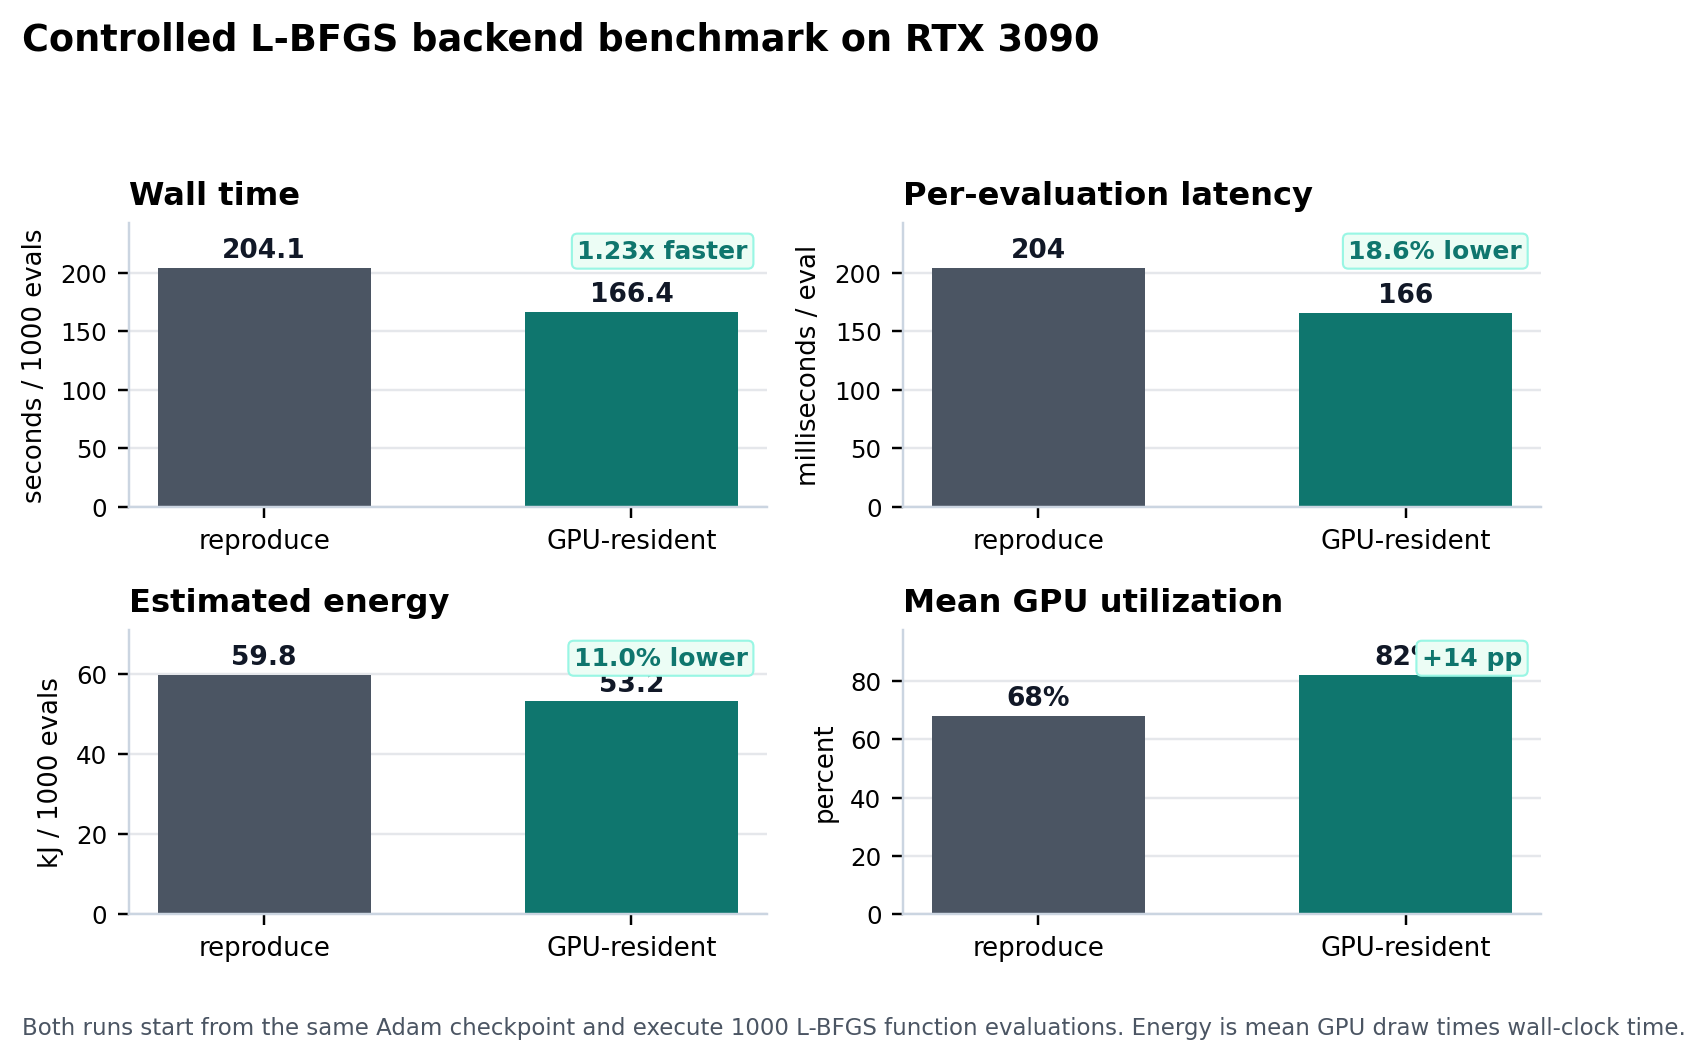
\includegraphics[width=\linewidth]{figures/lbfgs_backend_benchmark.png}
  \caption{Controlled backend comparison for $1000$ L-BFGS evaluations.
           The GPU-resident backend reduces wall-clock time, per-evaluation
           latency, and estimated energy while increasing mean GPU
           utilization.}
  \label{fig:backend_bench}
\end{figure}

The early-time snapshots ($t=0.10$--$0.20$~s) exhibit elevated errors
in both methods because the pulsatile inlet imposes the most rapid
variation; the PINN must satisfy a stiff constraint between the initial
condition ($u=v=0$ at $t=0$) and the imposed inlet profile, which is a
known source of difficulty for time-domain PINNs~\cite{wang2024causal}.

Pressure error is included after spatial demeaning to remove the arbitrary
pressure gauge.  The mean pressure errors are comparable
($10.79\%$ for \emph{reproduce} and $10.31\%$ for
\emph{GPU-resident}), although the final snapshot has a large pressure error
in both runs.  We therefore use pressure as a secondary diagnostic rather
than as the primary ranking criterion.

\todo{fig: field comparison of u, v, p at t=0.3, 0.4, 0.5 s for
GPU-resident vs reproduce vs Chorin reference (rainbow colormap, cylinder masked)}

% -----------------------------------------------------------------------
% Section: Results — Causal training (Re=10)
% -----------------------------------------------------------------------

\subsection{Causal Training}

To test whether temporal-causality weighting improves the transient
solution, we replace the PDE-residual term with the causally-weighted
form of Wang et al.~\cite{wang2024causal}.  The collocation points are
binned into $M=32$ equal-duration temporal slices, and bin $i$ receives a
stop-gradient weight
\begin{equation}
  w_i = \exp\!\Big(-\tfrac{\epsilon}{M}\textstyle\sum_{k<i} L_k\Big),
  \label{eq:causal_weight}
\end{equation}
where $L_k$ is the mean residual of bin $k$.  The exponent is normalized
by $M$ so that $\epsilon$ is independent of the bin count, and at
$\epsilon=0$ the loss reduces exactly to the unweighted residual of
Eq.~\eqref{eq:l2rel}'s underlying objective.  After the Adam phase the bin
weights are frozen as static constants during the L-BFGS phase, keeping
the quasi-Newton objective stationary.  We compare this \emph{frozen}
polish against a \emph{uniform} polish that instead optimises the
unweighted true loss (all bins equally weighted) during the L-BFGS phase.

Table~\ref{tab:l2_causal} reports the developed-window error
($t\geq0.1$~s) for causal Adam initialisations at $\epsilon\in\{30,50\}$,
each polished with either a frozen-weight or a uniform-weight L-BFGS
phase, alongside the \emph{reproduce} and \emph{GPU-resident} baselines.

\begin{table*}[t]
  \centering
  \caption{$Re=10$ developed-flow error ($t\geq0.1$~s, 41 snapshots).
           \emph{Mean} is the per-snapshot relative $L_2$ averaged over the
           window; \emph{Global} is the Frobenius $L_2$ over all space--time
           points; \emph{Loss} is the final unweighted training loss
           (PDE residual ${}+{}$ BC/IC).  Causal runs use $M=32$ temporal
           bins; \emph{frozen} keeps the Adam-end causal weights during
           L-BFGS, while \emph{uniform} optimises the unweighted loss.
           Pressure is spatially demeaned.  Best per column in bold.}
  \label{tab:l2_causal}
  \begin{tabular}{@{}l c ccc ccc@{}}
    \toprule
    & & \multicolumn{3}{c}{Mean $L_2$ (\%)} & \multicolumn{3}{c}{Global $L_2$ (\%)} \\
    \cmidrule(lr){3-5}\cmidrule(lr){6-8}
    Run & Loss & $\varepsilon_u$ & $\varepsilon_v$ & $\varepsilon_p$
        & $\varepsilon_u$ & $\varepsilon_v$ & $\varepsilon_p$ \\
    \midrule
    reproduce (baseline) & $2.1{\times}10^{-4}$ & 5.30 & 19.86 & 10.79 & 4.47 & 14.75 & 27.92 \\
    GPU-resident         & $2.9{\times}10^{-3}$ & 5.94 & 22.23 & 10.31 & 4.75 & 16.44 & 24.42 \\
    \midrule
    causal $\epsilon{=}30$, frozen  & $2.3{\times}10^{-4}$ & 5.22 & 20.38 & 11.03 & 4.36 & 15.02 & 28.49 \\
    causal $\epsilon{=}30$, uniform & $\mathbf{1.5{\times}10^{-4}}$ & \textbf{4.64} & \textbf{18.60} & \textbf{8.89} & \textbf{3.93} & \textbf{13.28} & \textbf{22.51} \\
    causal $\epsilon{=}50$, frozen  & $2.1{\times}10^{-4}$ & 5.34 & 19.86 & 10.10 & 4.47 & 15.05 & 25.83 \\
    causal $\epsilon{=}50$, uniform & $1.5{\times}10^{-4}$ & 4.96 & 19.21 & 9.70 & 4.14 & 13.93 & 25.30 \\
    \bottomrule
  \end{tabular}
\end{table*}

Two findings stand out.  First, at both $\epsilon$ values the
\emph{uniform} L-BFGS polish consistently beats the \emph{frozen} polish
on every field: at $\epsilon=50$ the velocity errors drop from
$5.34\%/19.86\%$ (frozen) to $4.96\%/19.21\%$ (uniform), and the
unweighted true loss is also lower ($1.5\times10^{-4}$ versus
$2.1\times10^{-4}$).  A causal Adam phase supplies a good initialisation,
but the subsequent L-BFGS reaches a more accurate field when it optimises
all temporal bins equally rather than retaining the causal
down-weighting of late times.  Second, the best configuration---causal
$\epsilon=30$ with a uniform polish ($\varepsilon_u=4.64\%$,
$\varepsilon_v=18.60\%$)---surpasses the \emph{reproduce} baseline
($5.30\%/19.86\%$) and approaches the original Rao TF checkpoint
($4.75\%/18.47\%$), even though that checkpoint cannot be reproduced.

These results are exploratory, not a controlled ablation.  The causal
runs use a more aggressive schedule ($20{,}000$ Adam iterations at
learning rate $10^{-3}$ with a plateau scheduler) than the baselines, so
the gain conflates the causal weighting with the longer, scheduled Adam
phase; an iso-budget sweep ($\epsilon\in\{0,2,5\}$ under matched settings)
is still required to isolate the causal-weighting contribution.
\todo{add iso-budget causal ablation ($\epsilon=0/2/5$, config matched to
the baselines) to separate the causal-weighting effect from the schedule}
We also note that the causal curriculum did not fully propagate within the
Adam budget ($\min_i w_i\approx0.77$--$0.85$), and that $\epsilon=30$ and
$\epsilon=50$ converged to nearly identical loss, so $\epsilon$ is weakly
determined in this regime.

\todo{fig: causal weight profile and $\min_i w_i$ vs.\ iteration
(results/figures/causal\_eps50\_adam20k/causal\_weight\_curve.png)}


\section{Conclusion}
\todo{USER: write conclusion — summarize Re=10 fidelity, gaps vs Rao pickle, planned extensions (Re=100, architecture ablation)}

\bibliographystyle{IEEEtran}
\bibliography{reference}

\end{document}
